\documentclass{beamer}

\usepackage[brazil]{babel}
\usepackage[utf8]{inputenc}

\usepackage{graphicx}
\usepackage{caption}
\usepackage{subcaption}

\usetheme{CambridgeUS}
\usecolortheme{dolphin}

\title[]{Cooperative Transport of Objects using Heterogeneous Robots}
\author[Ramon Soares de Melo]{
Ramon Soares de Melo\\Douglas G. Macharet\\Mario Fernando Montenegro Campos
}
\institute[]
{
  Instituto de Ciências Exatas - ICEx\\
  Laboratório de Visão Computacional e Robótica - VerLab\\
  Universidade Federal de Minas Gerais
}
\date{2015}
\subject{Computer Science}

\begin{document}

    
\newcommand{\mrs}{MRS}
\newcommand{\environment}{\ensuremath{\mathbb{R}^3}}

% Shortcut definitions

\newcommand{\set}[1]{\ensuremath{\boldsymbol{\mathcal{#1}}}}
\newcommand{\setitem}[2]{\ensuremath{#1_{#2}}}
\newcommand{\setlist}[3]{#1\ $=$\ \{\setitem{#2}{1}, \setitem{#2}{2}, ..., \setitem{#2}{#3}\}}

\newcommand{\robotset}{\set{R}} % conjunto de robôs
\newcommand{\robotsetqt}{\ensuremath{k}}
\newcommand{\robot}[1]{\setitem{r}{#1}}
\newcommand{\robotlist}{\setlist{\robotset}{r}{\robotsetqt}}

\newcommand{\obstacleset}{\set{B}} % conjunto de obstáculos
\newcommand{\obstaclesetqt}{\ensuremath{x}}
\newcommand{\obstacle}[1]{\setitem{b}{#1}}
\newcommand{\obstaclelist}{\setlist{\obstacleset}{b}{\obstaclesetqt}}

\newcommand{\objectset}{\set{O}} % conjunto de objetos
\newcommand{\objectsetqt}{\ensuremath{y}}
\newcommand{\object}[1]{\setitem{o}{#1}}
\newcommand{\objectlist}{\setlist{\objectset}{o}{\objectsetqt}}

\newcommand{\planset}{\set{P}} % plano
\newcommand{\plansetqt}{\ensuremath{q}}
\newcommand{\plan}[1]{\setitem{n}{#1}}
\newcommand{\planlist}{\setlist{\planset}{n}{\plansetqt}}

\newcommand{\robotplanset}{\set{RP}} % conjunto de planos
\newcommand{\robotplansetqt}{\ensuremath{j}}
\newcommand{\robotplan}[1]{\setitem{rp}{#1}}
\newcommand{\robotplanlist}{\setlist{\robotplanset}{rp}{\robotplansetqt}}

\newcommand{\executionplanset}{\set{EP}} % conjunto de planos
\newcommand{\executionplansetqt}{\ensuremath{h}}
\newcommand{\executionplan}[1]{\setitem{ep}{#1}}
\newcommand{\executionplanlist}{\setlist{\executionplanset}{ep}{\executionplansetqt}}
\newcommand{\executionplanname}{\emph{Execution Plan}}
\newcommand{\executionplansetnotation}{\ensuremath{\executionplanset \subset \robotplanset}}

\newcommand{\executionplanminset}{\ensuremath{\executionplanset{*}}} % conjunto com custo minimo de segmentos

\newcommand{\segmentset}{\set{S}} % conjunto de segmentos
\newcommand{\segmentsetqt}{\ensuremath{e}}
\newcommand{\segment}[1]{\setitem{s}{#1}}
\newcommand{\segmentlist}{\setlist{\segmentset}{s}{\segmentsetqt}}

\newcommand{\segmentpointset}{\ensuremath{\set{S}_p}} % conjunto de pontos de segmentação
\newcommand{\segmentpointsetqt}{\ensuremath{z}}
\newcommand{\segmentpoint}[1]{\setitem{sp}{#1}}
\newcommand{\segmentpointfirst}[1]{\ensuremath{\segmentpoint{#1}^1}}
\newcommand{\segmentpointsecond}[1]{\ensuremath{\segmentpoint{#1}^2}}

\newcommand{\segmentpointlist}{\setlist{\segmentpointset}{sp}{\segmentpointsetqt}}

\newcommand{\typeland}{ground}
\newcommand{\typeaerial}{aerial}
\newcommand{\typeset}{\set{T}} % conjunto de tipos de movimentação
\newcommand{\typelist}{\ensuremath{\typeset=\ \{}\typeland, \typeaerial\ensuremath{\}}}
\newcommand{\type}[1]{\setitem{t}{#1}}

\newcommand{\plantypestart}{initial}
\newcommand{\plantypetransition}{transition}
\newcommand{\plantypemove}{movement}
\newcommand{\plantypeset}{\set{TP}} % conjunto de tipos de plano
\newcommand{\plantypelist}{\ensuremath{\plantypeset=\ \{}\plantypestart, \plantypetransition, \plantypemove\ensuremath{\}}}
\newcommand{\plantype}[1]{\setitem{tp}{#1}}

\newcommand{\movementtypepremove}{pre-transport}
\newcommand{\movementtypemove}{transport}
\newcommand{\movementtypeset}{\set{T_m}} % conjunto de tipos de plano
\newcommand{\movementtypelist}{\ensuremath{\movementtypeset=\ \{}\movementtypepremove, \movementtypemove\ensuremath{\}}}
\newcommand{\movementtype}[1]{\setitem{tm}{#1}}

\newcommand{\tokenset}{\set{TO}}
\newcommand{\tokensetqt}{\ensuremath{u}}
\newcommand{\tokeni}[1]{\setitem{to}{#1}}
\newcommand{\token}{\emph{token}}
\newcommand{\tokenlist}{\setlist{\tokenset}{to}{\tokensetqt}}

\newcommand{\workspace2}{\ensuremath{\boldsymbol{\mathcal{W}}}} % àrea de trabalho
\newcommand{\workspacecell}{\ensuremath{\boldsymbol{\mathcal{c}}}} % àrea de trabalho

\newcommand{\allocationgraph}{\ensuremath{\mathcal{AG}}}
\newcommand{\allocationgraphcompress}{\ensuremath{\mathcal{AG}_c}}

\newcommand{\currentstate}{\ensuremath{S}}
\newcommand{\nextstate}{\ensuremath{S'}}
\newcommand{\originstate}{\ensuremath{S_o}}
\newcommand{\targetstate}{\ensuremath{S_d}}
\newcommand{\robotstate}{\ensuremath{S_r}}

\newcommand{\robotinitialstate}{\ensuremath{I}}
\newcommand{\robotinitialstatei}[1]{\ensuremath{I_{#1}}}

\newcommand{\celldimension}{\ensuremath{d}}
\newcommand{\deslocationfactor}{\ensuremath{l}}

\newcommand{\movementset}{\set{M}}
\newcommand{\movementslist}{\ensuremath{\movementset=\ \{}left, right, front, back, up, down\ensuremath{\}}}
\newcommand{\movementaction}{\ensuremath{a_i}}

% Funções

\newcommand{\utilityfunction}{\ensuremath{\Theta}}
\newcommand{\utilityplanfunction}{\ensuremath{\utilityfunction_{p}}}
\newcommand{\utilitytotalfunction}{\ensuremath{\utilityfunction_{t}}}
\newcommand{\distancefunction}{\ensuremath{\Delta}}
\newcommand{\timefunction}{\ensuremath{\Upsilon}}
\newcommand{\energyfunction}{\ensuremath{\Psi}}

% Planejamento

\newcommand{\fringe}{\set{F}}
\newcommand{\searchednodes}{\set{SN}}
\newcommand{\node}{\ensuremath{n}}
\newcommand{\nodeitem}[1]{\ensuremath{\node_{#1}}}
\newcommand{\nodeparent}{\emph{NodePai}}
\newcommand{\nodeutility}{\ensuremath{\omega}}
\newcommand{\nodedata}{\ensuremath{\{}state (\currentstate), action (\movementaction), utility (\nodeutility), agent's position (\robotstate), type (\type{i})\ensuremath{\}}}


    \begin{frame}
        \titlepage
    \end{frame}

    % \begin{frame}
    %     \frametitle{Table of Contents}
    %     \tableofcontents[currentsection]
    % \end{frame}

    % Aplicações do robots
    % Transporte e manipulação
    % Trabalhos relacionados
    %

    \section{Introduction} % (fold)
    \label{sec:introdu_o}

    % \frame{
    %     \frametitle{Aplicações dos Robôs}

    %     \begin{figure}[p]

    %         \centering
    %         \begin{subfigure}[b]{0.24\textwidth}
    %             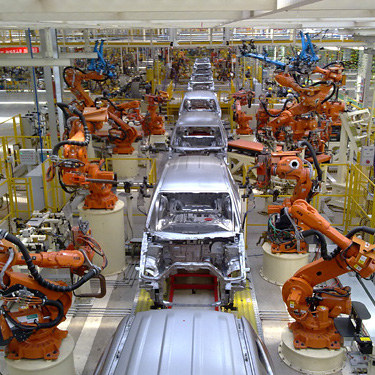
\includegraphics[width=\textwidth]{imgs/linha_montagem.jpg}
    %             \caption*{Manufatura}
    %         \end{subfigure}
    %         \begin{subfigure}[b]{0.24\textwidth}
    %             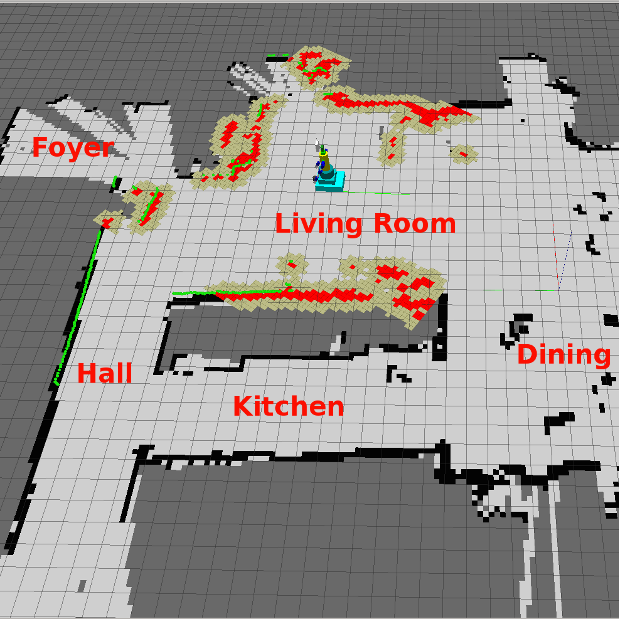
\includegraphics[width=\textwidth]{imgs/mapeamento.png}
    %             \caption*{Mapeamento}
    %         \end{subfigure}
    %         \begin{subfigure}[b]{0.24\textwidth}
    %             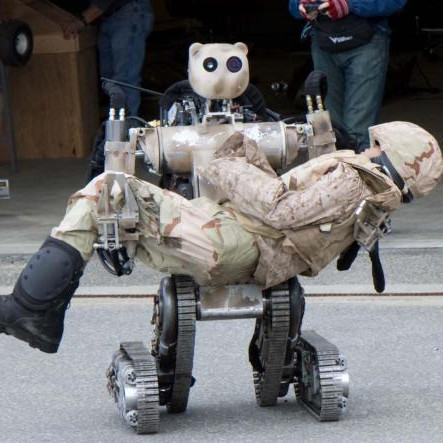
\includegraphics[width=\textwidth]{imgs/resgate.jpg}
    %             \caption*{Resgate}
    %         \end{subfigure}\\
    %         \begin{subfigure}[b]{0.24\textwidth}
    %             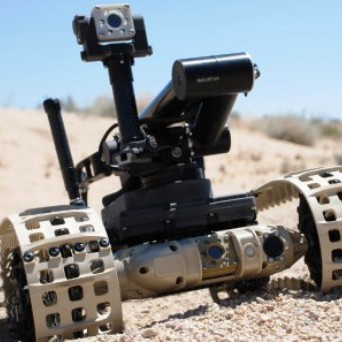
\includegraphics[width=\textwidth]{imgs/vigilancia.jpg}
    %             \caption*{Vigilância}
    %         \end{subfigure}
    %         \begin{subfigure}[b]{0.24\textwidth}
    %             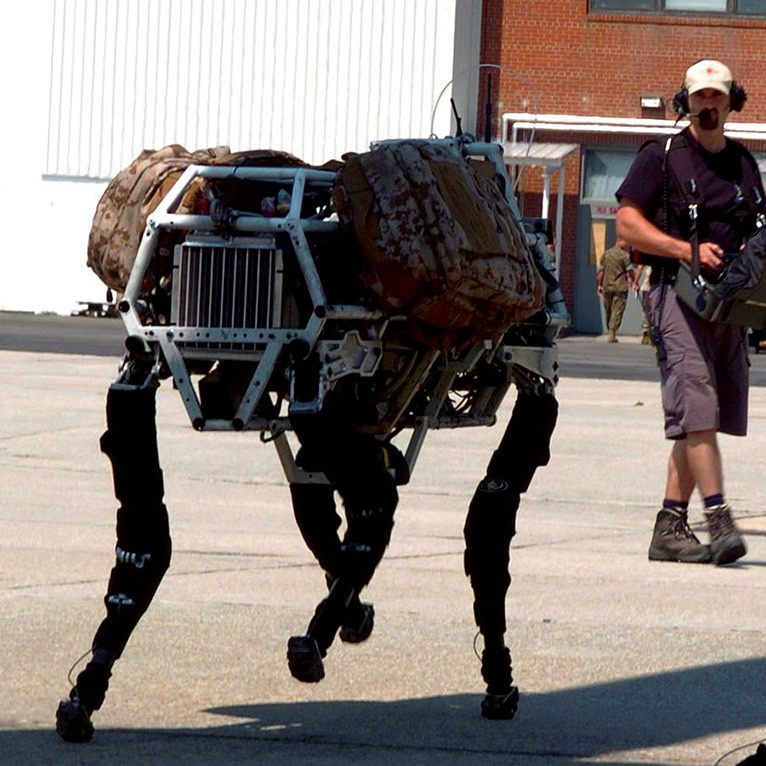
\includegraphics[width=\textwidth]{imgs/transport.jpg}
    %             \caption*{Transporte}
    %         \end{subfigure}
    %     \end{figure}
    % }

    % \frame{
    %     \frametitle{Classificação quanto número de Agentes}

    %     \begin{description}
    %         \item[Único Agente] Caso no qual a missão é planejada e executada utilizando somente um agente, que deve ser capaz de realizá-la completamente e possuir todas as capacidades necessárias.

    %         % somente um agente pode falhar, além do mesmo ter de ser muito complexo em alguns casos

    %         \vspace{0.2cm}

    %         \item[Multi-Agente] Sistema munido de vários agentes disponíveis para realizar a tarefa, podendo cada agente possuir diferentes recursos e capacidades.

    %         % se um dos agentes falar, outros podem tomar o seu lugar e completar a missão

    %     \end{description}
    % }

    % \frame{
    %     \frametitle{Multi-Agentes}

    %     \begin{description}
    %         \item[Vantagens]
    %         \begin{itemize}
    %             \item Maior tolerância a falhas;
    %             \item Podem reduzir o tempo total de execução da tarefa;
    %             \item Executar tarefas complexas com agentes simples.
    %         \end{itemize}
    %         \vspace{0.5cm}
    %         \item[Dificuldades]
    %         \begin{itemize}
    %             \item Planejamento de Caminhos;
    %             \item Alocação de Tarefas;
    %             \item Coordenação.
    %         \end{itemize}
    %     \end{description}
    % }

    \subsection{Motivation} % (fold)
    \label{sub:motiva_o}

    \frame{
        \frametitle{Object Manipulation}

        Transport and manipulation of objects is a basic task in other actions:

        \begin{figure}[p]

            \centering
            \begin{subfigure}[b]{0.24\textwidth}
                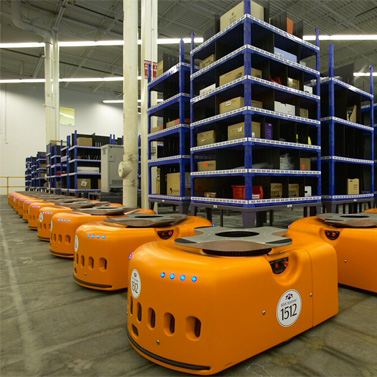
\includegraphics[width=\textwidth]{imgs/transporte1.png}
                \caption*{Transport}
            \end{subfigure}
            \begin{subfigure}[b]{0.24\textwidth}
                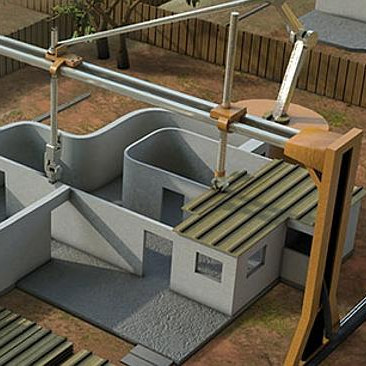
\includegraphics[width=\textwidth]{imgs/transporte2.jpg}
                \caption*{Construction}
            \end{subfigure}
            \begin{subfigure}[b]{0.24\textwidth}
                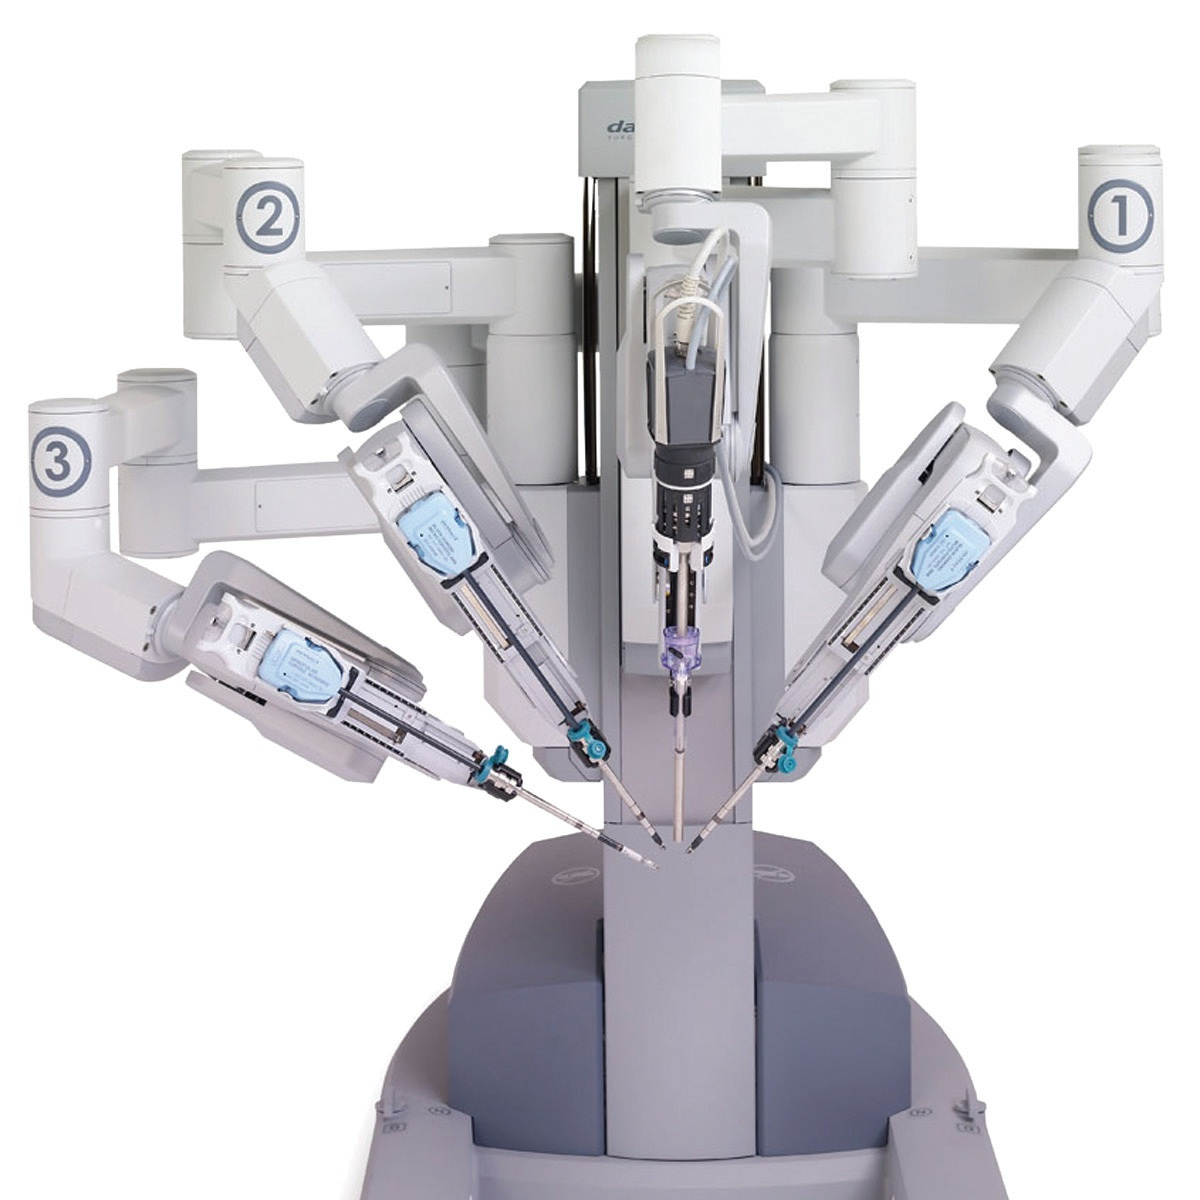
\includegraphics[width=\textwidth]{imgs/transporte3.jpg}
                \caption*{Tools}
            \end{subfigure}
            \begin{subfigure}[b]{0.24\textwidth}
                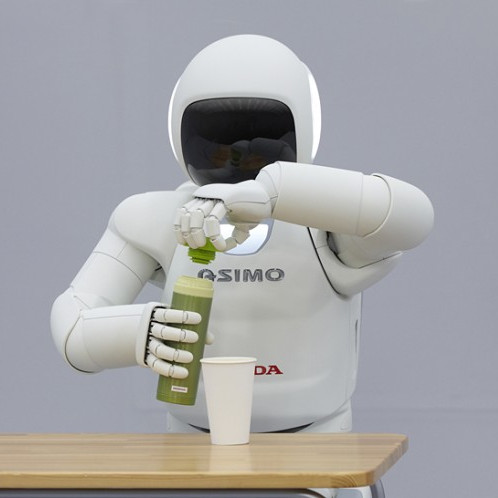
\includegraphics[width=\textwidth]{imgs/transporte4.jpg}
                \caption*{Household Usage}
            \end{subfigure}

        \end{figure}
    }

    % subsection motiva_o (end)

    \subsection{Problem} % (fold)
    \label{sub:problema}

    \frame{
        \frametitle{Problem Definition}

        \begin{columns}[c]
          \begin{column}{0.7\textwidth}

            \textbf{Problem 1} \textit{Object Path Planning}
            \vspace{0.2cm}\\
            Find a feasible path inside the workspace to each object, starting from its initial position until a desired end position.

          \end{column}
          \begin{column}{0.3\textwidth}
            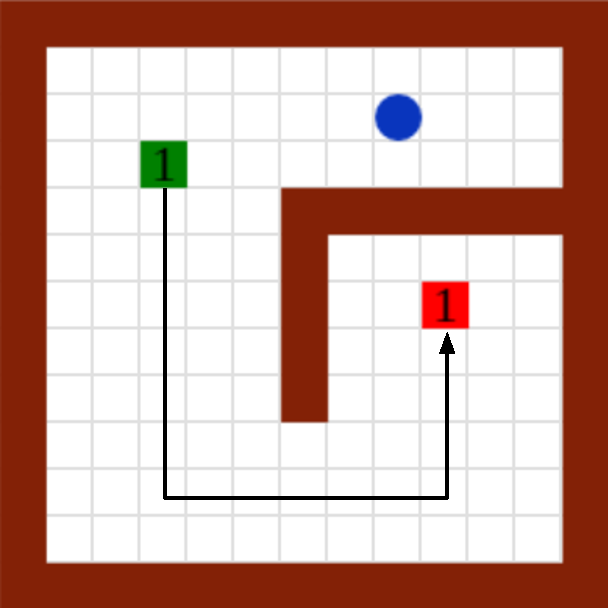
\includegraphics[width=\textwidth]{imgs/MoveIntro_1.pdf}
          \end{column}
        \end{columns}

        \begin{columns}[c]
          \begin{column}{0.7\textwidth}

            \textbf{Problem 2} \textit{Agents Coordination}
            \vspace{0.2cm}\\
            Allocate and Coordinate agents to accomplish each required path of the objects.


          \end{column}
          \begin{column}{0.3\textwidth}
            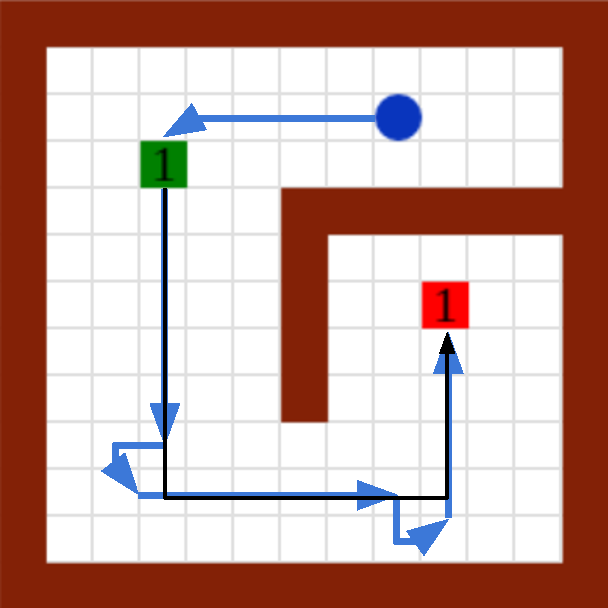
\includegraphics[width=\textwidth]{imgs/MoveIntro_2.pdf}
          \end{column}
        \end{columns}


        % \begin{quotation}
        %     Seja \workspace\ uma área de trabalho definida como $\workspace \subset \environment$, são definidos os conjuntos: (i) \objectlist, possuindo os objetos a serem transportados, (ii) \obstaclelist, contendo obstáculos em \workspace\ e (iii) \robotlist, com todos os agentes disponíveis para a tarefa de transporte.
        % \end{quotation}

        % \begin{description}
        %     \item[Problema 1] (Planejamento de Caminhos do Objeto) \emph{Dado o ambiente de trabalho \workspace, estudar e descrever uma sequência de poses válidas para os objetos em \objectset\ que garantam a chegada do mesmo à sua posição final desejada.}

        %     \item[Problema 2] (Alocação de Tarefas e Coordenação de Agentes) \emph{Tendo como base os planos de manipulação dos objetos, gerar uma distribuição de tarefas entre os agentes disponíveis e coordená-los de modo que executem o transporte dos objetos.}
        % \end{description}
    }

    % subsection problema (end)

    % section introdu_o (end)

    % \section{Trabalhos Relacionados} % (fold)
    % \label{sec:trabalhos_relacionados}

    % \frame{
    %     \frametitle{Trabalhos Relacionados}

    %     \begin{itemize}
    %         \item CoMutaR: A framework for multi-robot coordination and task allocation \cite{Shiroma2009};
    %         \item Optimal bid valuation using path finding for multi-robot task allocation \cite{Oeztuerk2014};
    %         \item A Multi-robot Exploration Approach Based on Distributed Graph Coloring \cite{Carvalho2013};
    %         \item A fast and frugal method for team-task allocation in a multi-robot transportation system \cite{Wawerla2010}.
    %     \end{itemize}
    % }

    % section trabalhos_relacionados (end)

    \section{Metodology} % (fold)
    \label{sec:metodologia}

    \frame{
        \frametitle{Metodology}

        \begin{figure}[p]
            \centering
            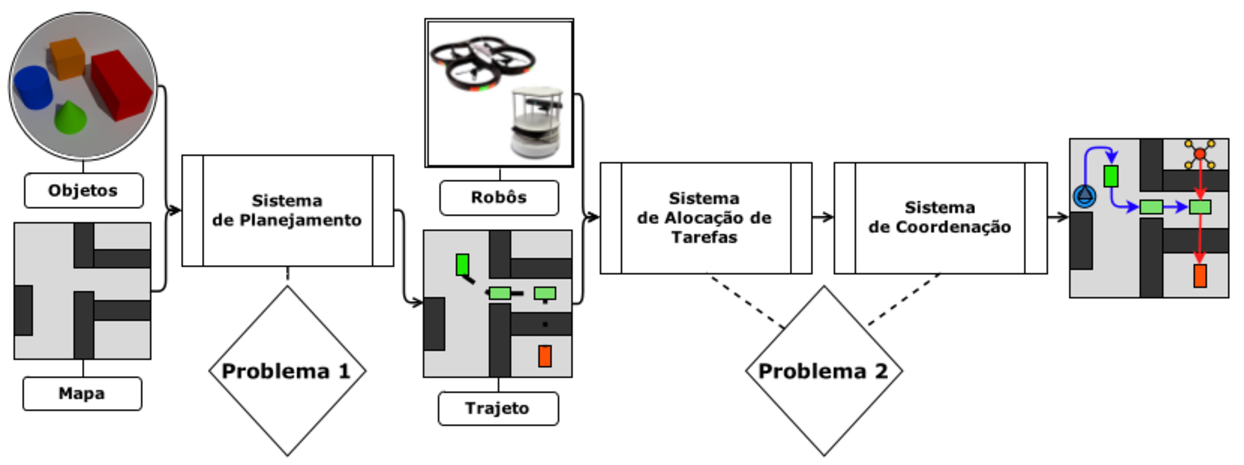
\includegraphics[width=\textwidth]{imgs/DiagramaGeral.pdf}
            \caption*{Metodology Diagram}
        \end{figure}
    }

    \frame{
        \frametitle{Utility Function}

        Quantifies the quality of a plan based on the energy and the drive time of a robot.
        % Quantifica a qualidade de um plano considerando as dimensões: distância (\distancefunction), tempo (\timefunction) e energia (\energyfunction). Utilizada para comparar e selecionar os melhores planos para o transporte.

        \begin{equation}
            \utilityfunction(\currentstate, \robot{i}) = \beta \times \timefunction(\currentstate, \robot{i}) + \gamma \times \energyfunction(\currentstate, \robot{i}).
            \label{eq:util_function}
        \end{equation}

        \begin{equation}
            \utilityplanfunction(\planset) = \sum\limits_{i=1}^\plansetqt \utilityfunction(\plan{i})
            \label{eq:plan_util_function}
        \end{equation}

        \let\thefootnote\relax\footnotetext{\currentstate: current state, \robot: robot, \planset: plan}
    }

    \frame{
        \frametitle{Path Planning - Object}

        \begin{columns}[c]

            \begin{column}[c]{0.5\textwidth}
                Planning for a object from set \objectset\ has two phases:

                \begin{enumerate}
                    \item \emph{Planning}: a travel plan is created;
                    \vspace{0.2cm}
                    \item \emph{Segmentation}: the plan is splitted into sub-plans.
                \end{enumerate}
            \end{column}

            \begin{column}[c]{0.5\textwidth}
                \begin{figure}[p]
                    \centering
                    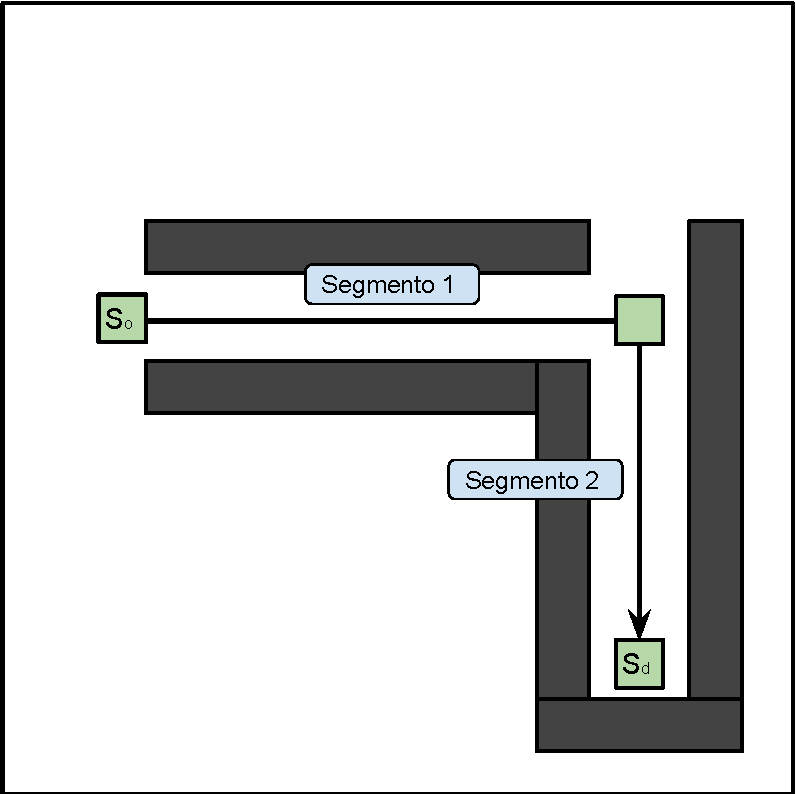
\includegraphics[width=0.9\textwidth]{imgs/ObjectMovement.pdf}
                    \caption*{Object Plan}
                \end{figure}
            \end{column}

        \end{columns}

        \let\thefootnote\relax\footnotetext{\originstate: initial state, \targetstate: end state}
    }

    \frame{
        \frametitle{Path Planning - Agents}

        \begin{columns}[c]

            \begin{column}[c]{0.5\textwidth}

                Based on segments created from the object's plan, for each agent \robot{i}, movimentation plans are created, of two types:

                \begin{itemize}
                    \item \emph{Preparation}: plan in which the robot approaches the object to be transported;
                    \vspace{0.2cm}
                    \item \emph{Transport}: plan used to transport the object.
                \end{itemize}


            \end{column}

            \begin{column}[c]{0.5\textwidth}
                \begin{figure}[p]
                    \centering
                    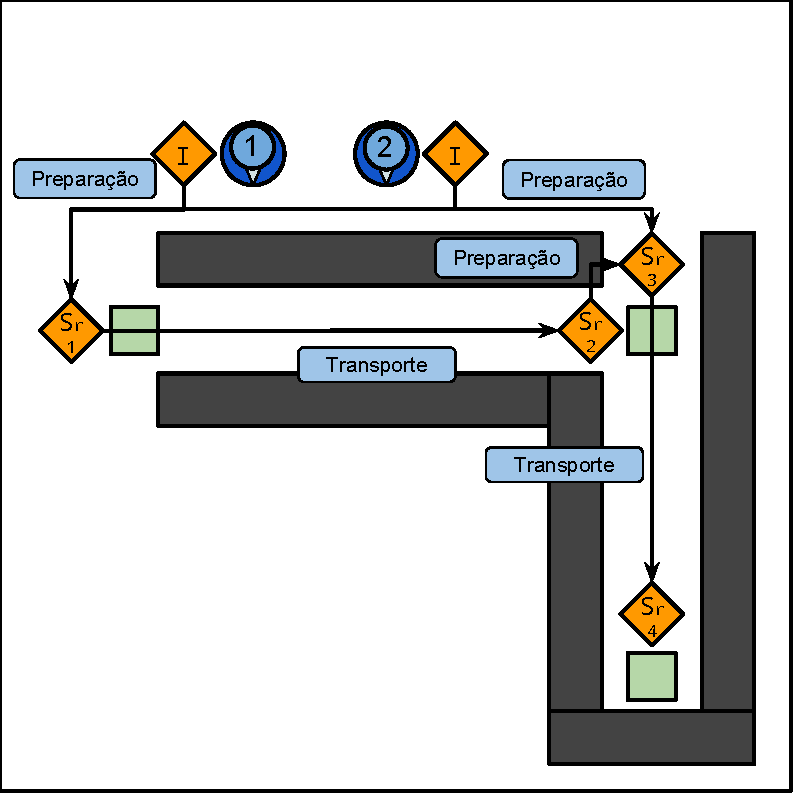
\includegraphics[width=0.9\textwidth]{imgs/RobotMovement.pdf}
                    \caption*{Agent's Plan}
                \end{figure}
            \end{column}

        \end{columns}
    }

    \frame{
        \frametitle{Task Allocation}

        \begin{columns}[c]

            \begin{column}[c]{0.5\textwidth}

                Task Allocation Process:

                \begin{enumerate}
                    \item Based on the object's plan, each robot create its own plan to transport it;
                    \item The robots exchange its cost plans, and apply the Hungarian Method the know which robot will do each plan;
                    \item Repeat the process until all object's plan are allocated.
                \end{enumerate}

            \end{column}

            \begin{column}[c]{0.5\textwidth}

                \begin{figure}[p]
                    \centering
                    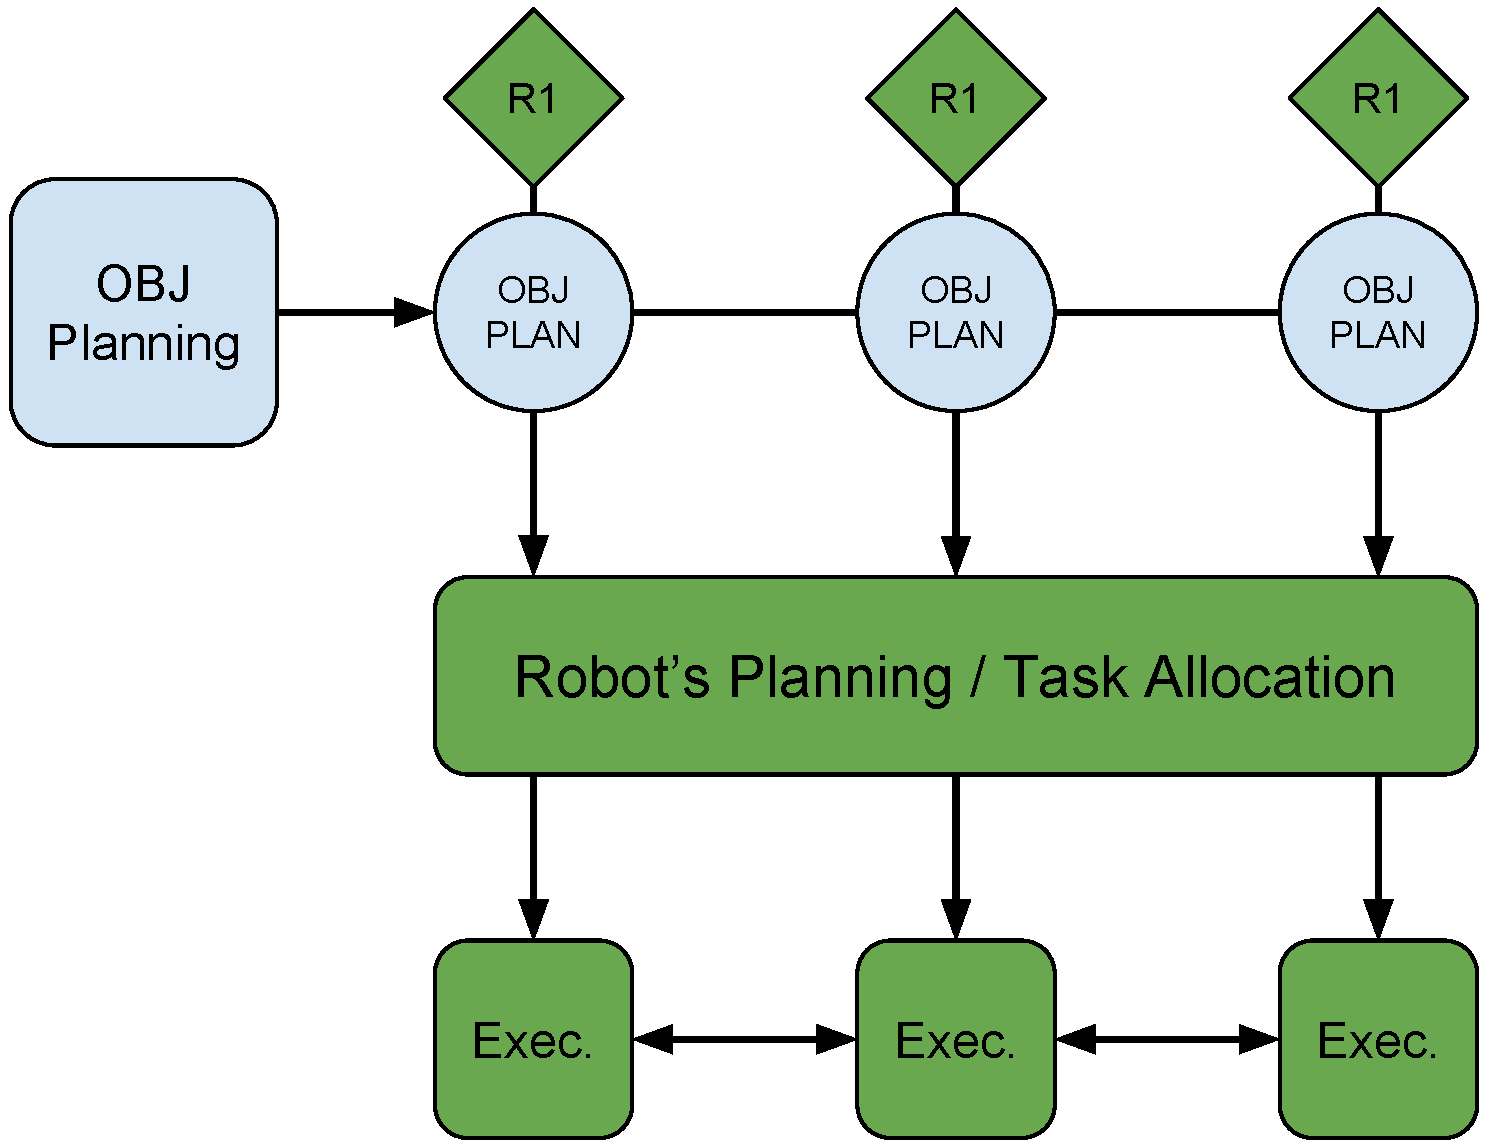
\includegraphics[width=\textwidth]{imgs/TaskAllocationProcess.pdf}
                    \caption*{Allocation Process}
                \end{figure}
            \end{column}

        \end{columns}
    }

    \frame{
        \frametitle{Coordination}

        The coordination process occurs with the exchange of information about the current task that each robot is executing.

        When a object is transported by multiple robots, they inform each other to wait until it's possible to execute their tasks.

        \begin{figure}[p]

            \centering
            \begin{subfigure}[b]{0.225\textwidth}
                \fbox{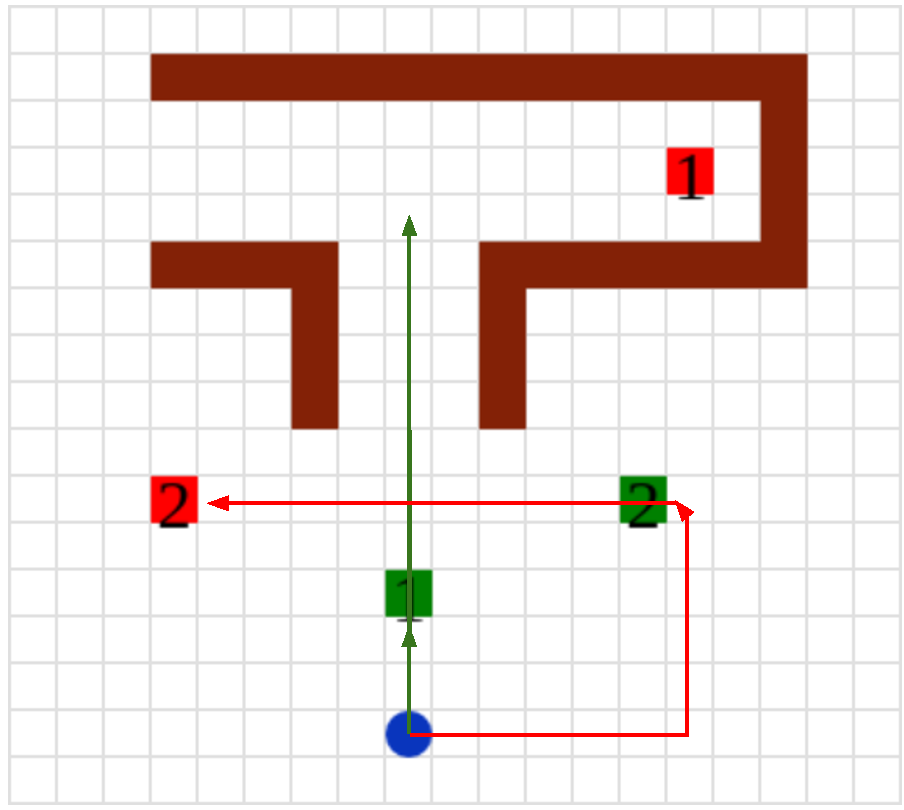
\includegraphics[width=\textwidth]{imgs/coordination/Mov1.pdf}}
                % \caption*{}
            \end{subfigure}
            \hspace{0.1cm}
            \begin{subfigure}[b]{0.225\textwidth}
                \fbox{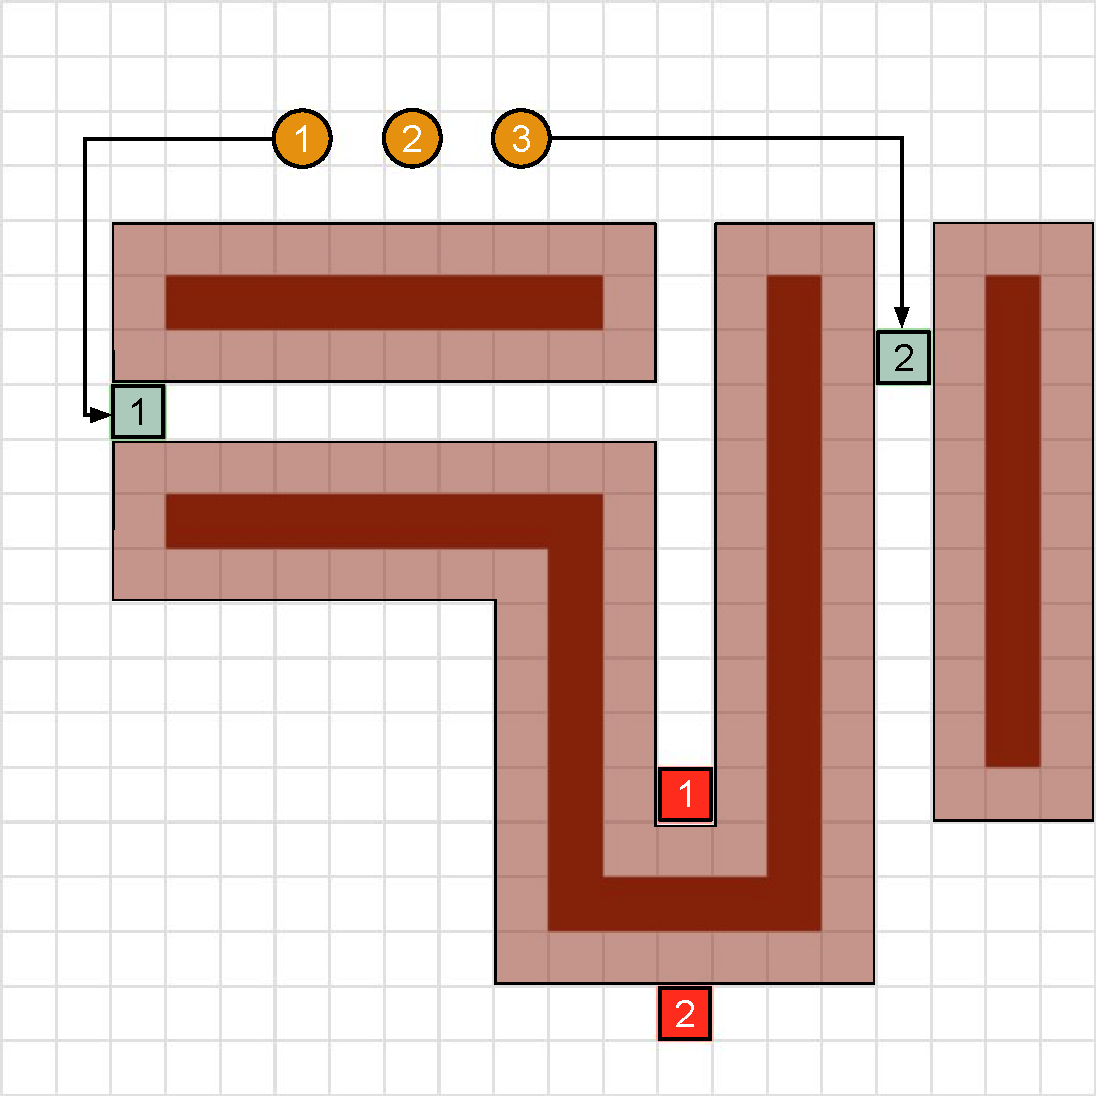
\includegraphics[width=\textwidth]{imgs/coordination/Mov2.pdf}}
                % \caption*{}
            \end{subfigure}
            \hspace{0.1cm}
            \begin{subfigure}[b]{0.225\textwidth}
                \fbox{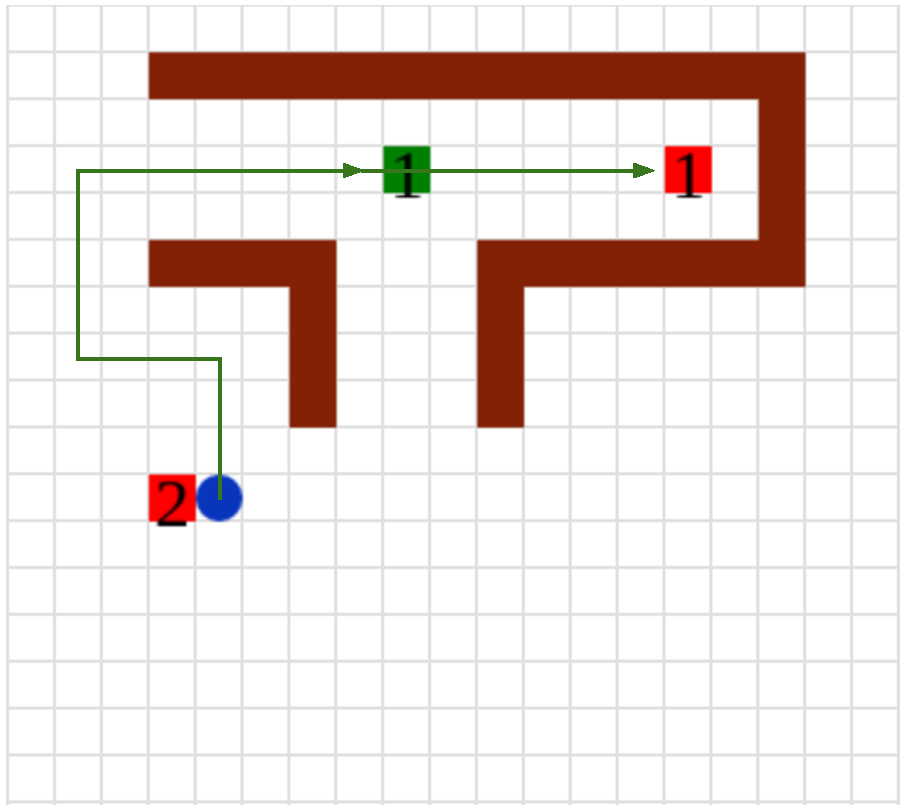
\includegraphics[width=\textwidth]{imgs/coordination/Mov3.pdf}}
                % \caption*{Tools}
            \end{subfigure}
            \hspace{0.1cm}
            \begin{subfigure}[b]{0.225\textwidth}
                \fbox{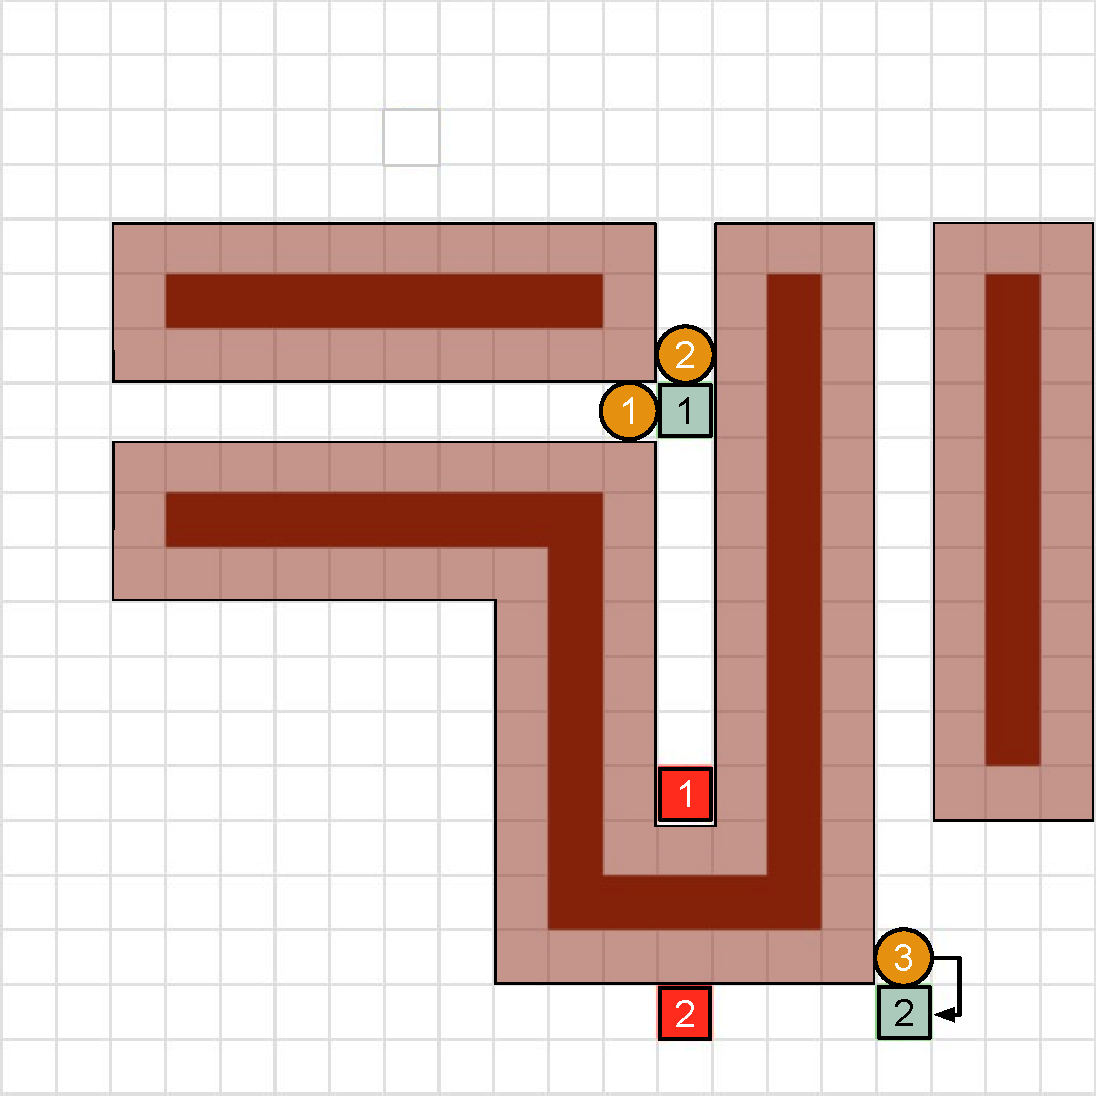
\includegraphics[width=\textwidth]{imgs/coordination/Mov4.pdf}}
                % \caption*{Household Usage}
            \end{subfigure}

        \end{figure}
    }

    % section metodologia (end)

    \section{Experiments} % (fold)
    \label{sec:experimentos}

    \frame{
        \frametitle{Experiments}

        \begin{figure}[p]
            \centering
            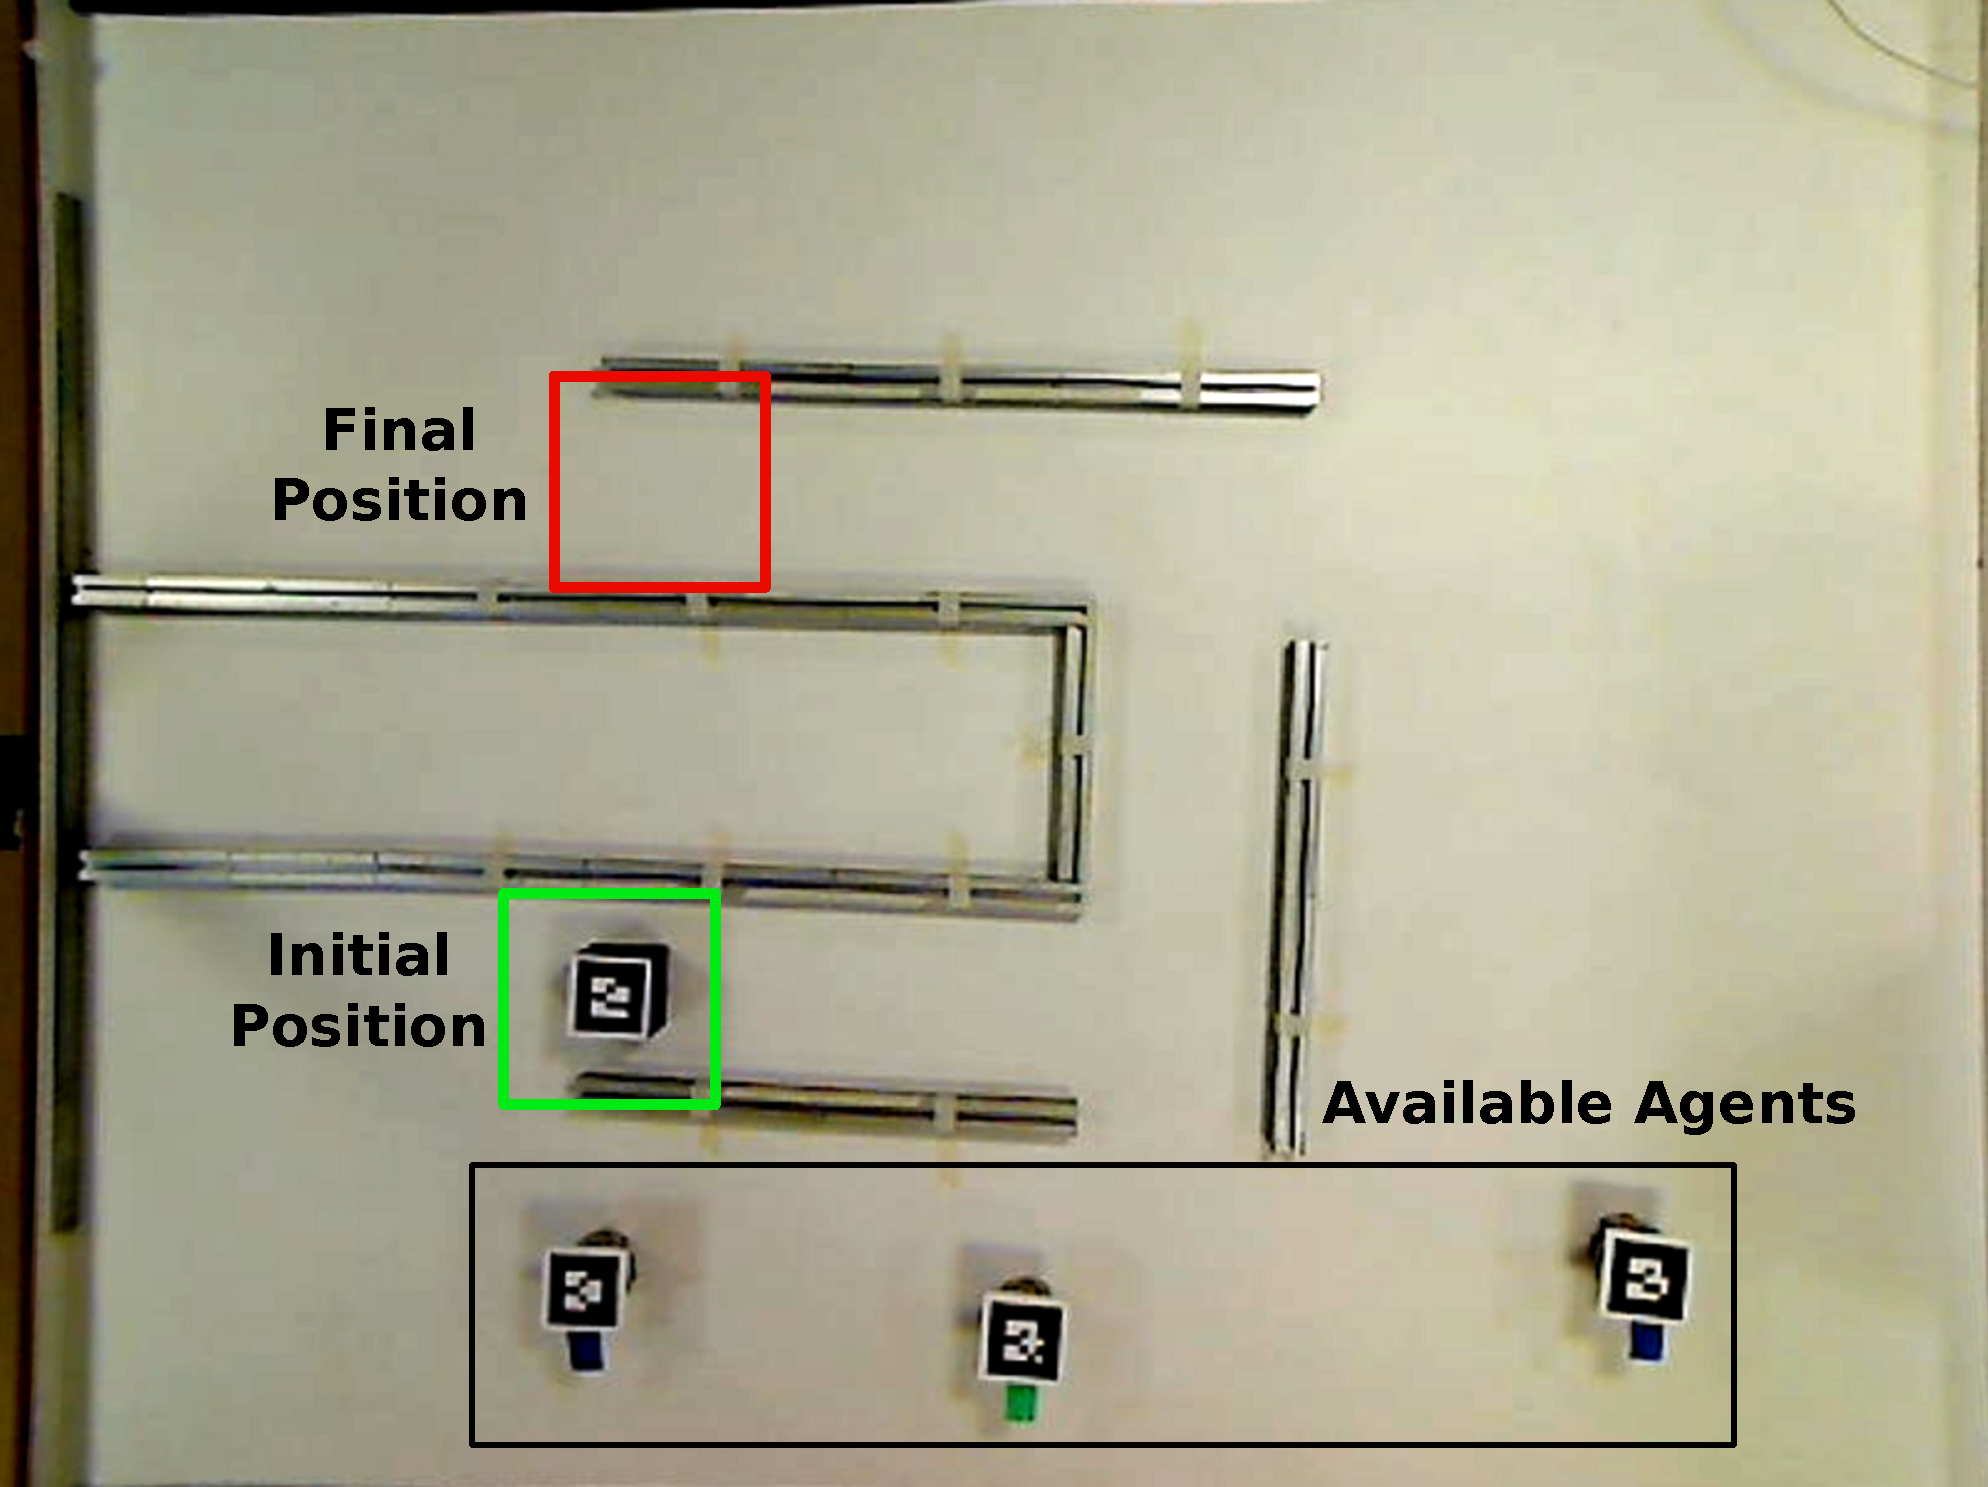
\includegraphics[width=0.75\textwidth]{imgs/experiment2.pdf}
        \end{figure}
    }

    % section experimentos (end)

\end{document}
